\section{DS1}
\subsection{Definition Biodiversität}
\textbf{Erste Nennung:} „National Forum of BioDiversity“ (Name einer Tagung 1986 in Washington, USA)\\
\textbf{Biodiversität = Information}\\
Components of biodiversity [nach Noss (1990)]
\begin{itemize}
	\item Compositional
	\begin{itemize}
		\item Genes
		\item Species, populations
		\item Communities/ecosystems
		\item Landscape type
	\end{itemize}
	\item Structural
	\begin{itemize}
		\item Landscape patterns
		\item Physiognomy/habitat structure
		\item Population structure
		\item Genetic structure
	\end{itemize}
	\item Functional
	\begin{itemize}
		\item Gentic process
		\item Demographis process
		\item Interspecific interactions
		\item Landscape process/disturbances
	\end{itemize}
\end{itemize}

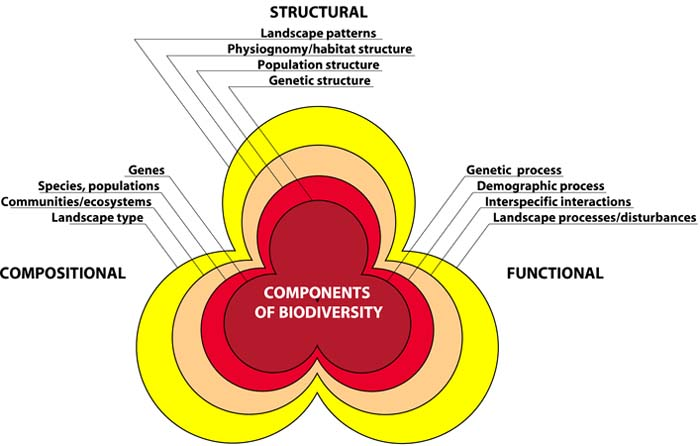
\includegraphics[width=0.8\textwidth]{lectures/DS1/pix/y5187e12.jpg}\\
http://www.fao.org/docrep/006/y5187e/y5187e12.jpg